\providecommand{\main}{..}
\documentclass[\main/main.tex]{subfiles}

\begin{document}
\graphicspath{{img/}{position_estimation/img/}}
\chapter{Position estimation}

In this chapter, a position estimation technique is introduced. The ultimate aim of this technique is to be simple enough to run on a microcontroller while providing reasonable accuracy. Section \ref{sec:distance_measurement_using_time_of_flight} discusses about a technique used for distance measurement. A solution for solving location from distance to known points is proposed in chapter \ref{sec:localization_using_trilateration}.

\section{Distance measurement using time-of-flight}
\label{sec:distance_measurement_using_time_of_flight}

\subsection{RSSI vs Time of Flight Distance Estimation}
Generally, there are two ways to measure distances between two devices. The first is based on RSSI, or Received Signal Strength Indication. We know that the signal strength drops with increasing distance from the transmitter in a deterministic fashion that is based on theoretic formulas. With this assumption, we can estimate the distance between a receiver and transmitter. However, this approach has several disadvantages. Since the environment and thus the radio channel changes constantly, then so does the RSSI parameter, which in turn brings inaccuracy to the system. The RSSI parameter can be also degraded by multipath propagation and other phenomenons that are quite common for the radio channel. The results and the overall accuracy can be increased by a process called fingerprinting, however due to rapidly changing radio environments, this process would need to be done frequently to improve the ranging results. Traditional technologies like Wi-Fi, Bluetooth, Bluetooth Low Energy and Active RFID are based on this distance estimation process.

Another option is to use the signal’s Time of Flight rather than RSSI. This yields much more accurate results in Line of Sight environments and can lead up to a centimeter level accuracy depending on the frequency and nature of the signal. This is an approach that is used by the Ultra Wideband technology. By combining the Time of Flight measurements from several devices, we can obtain an accurate position with precision of up to several centimeters. The nature of UWB signals makes it an ideal candidate for utilizing the Time of Flight distance estimation process. The performance might be degraded for example by obscuring the Line of Sight between UWB devices, however the overall accuracy is still superior in comparison to RSSI.

Time of Flight (ToF) is a method for measuring the distance between two radio transceivers by multiplying the Time of Flight of the signal by the speed of light. From this basic principle, UWB technology can be implemented in different ways based on the target applications needs: Two Way Ranging (TWR), Time Difference of Arrival (TDoA), or Phase Difference of Arrival (PDoA).

\subsection{Time Difference of Arrival (TDoA)}
The TDoA method is very similar to GPS. Multiple reference points, called anchors, are deployed in a venue and are time synchronized. The mobile devices will beacon, and when an anchor receives the beacon signal it will timestamp it. The timestamps from multiple anchors are then sent back to a central location engine which will run multilateration algorithms based on Time Difference of Arrival of the beacons signals to compute the X, Y, Z of the mobile devices.

\begin{figure}[H]
    \centering
    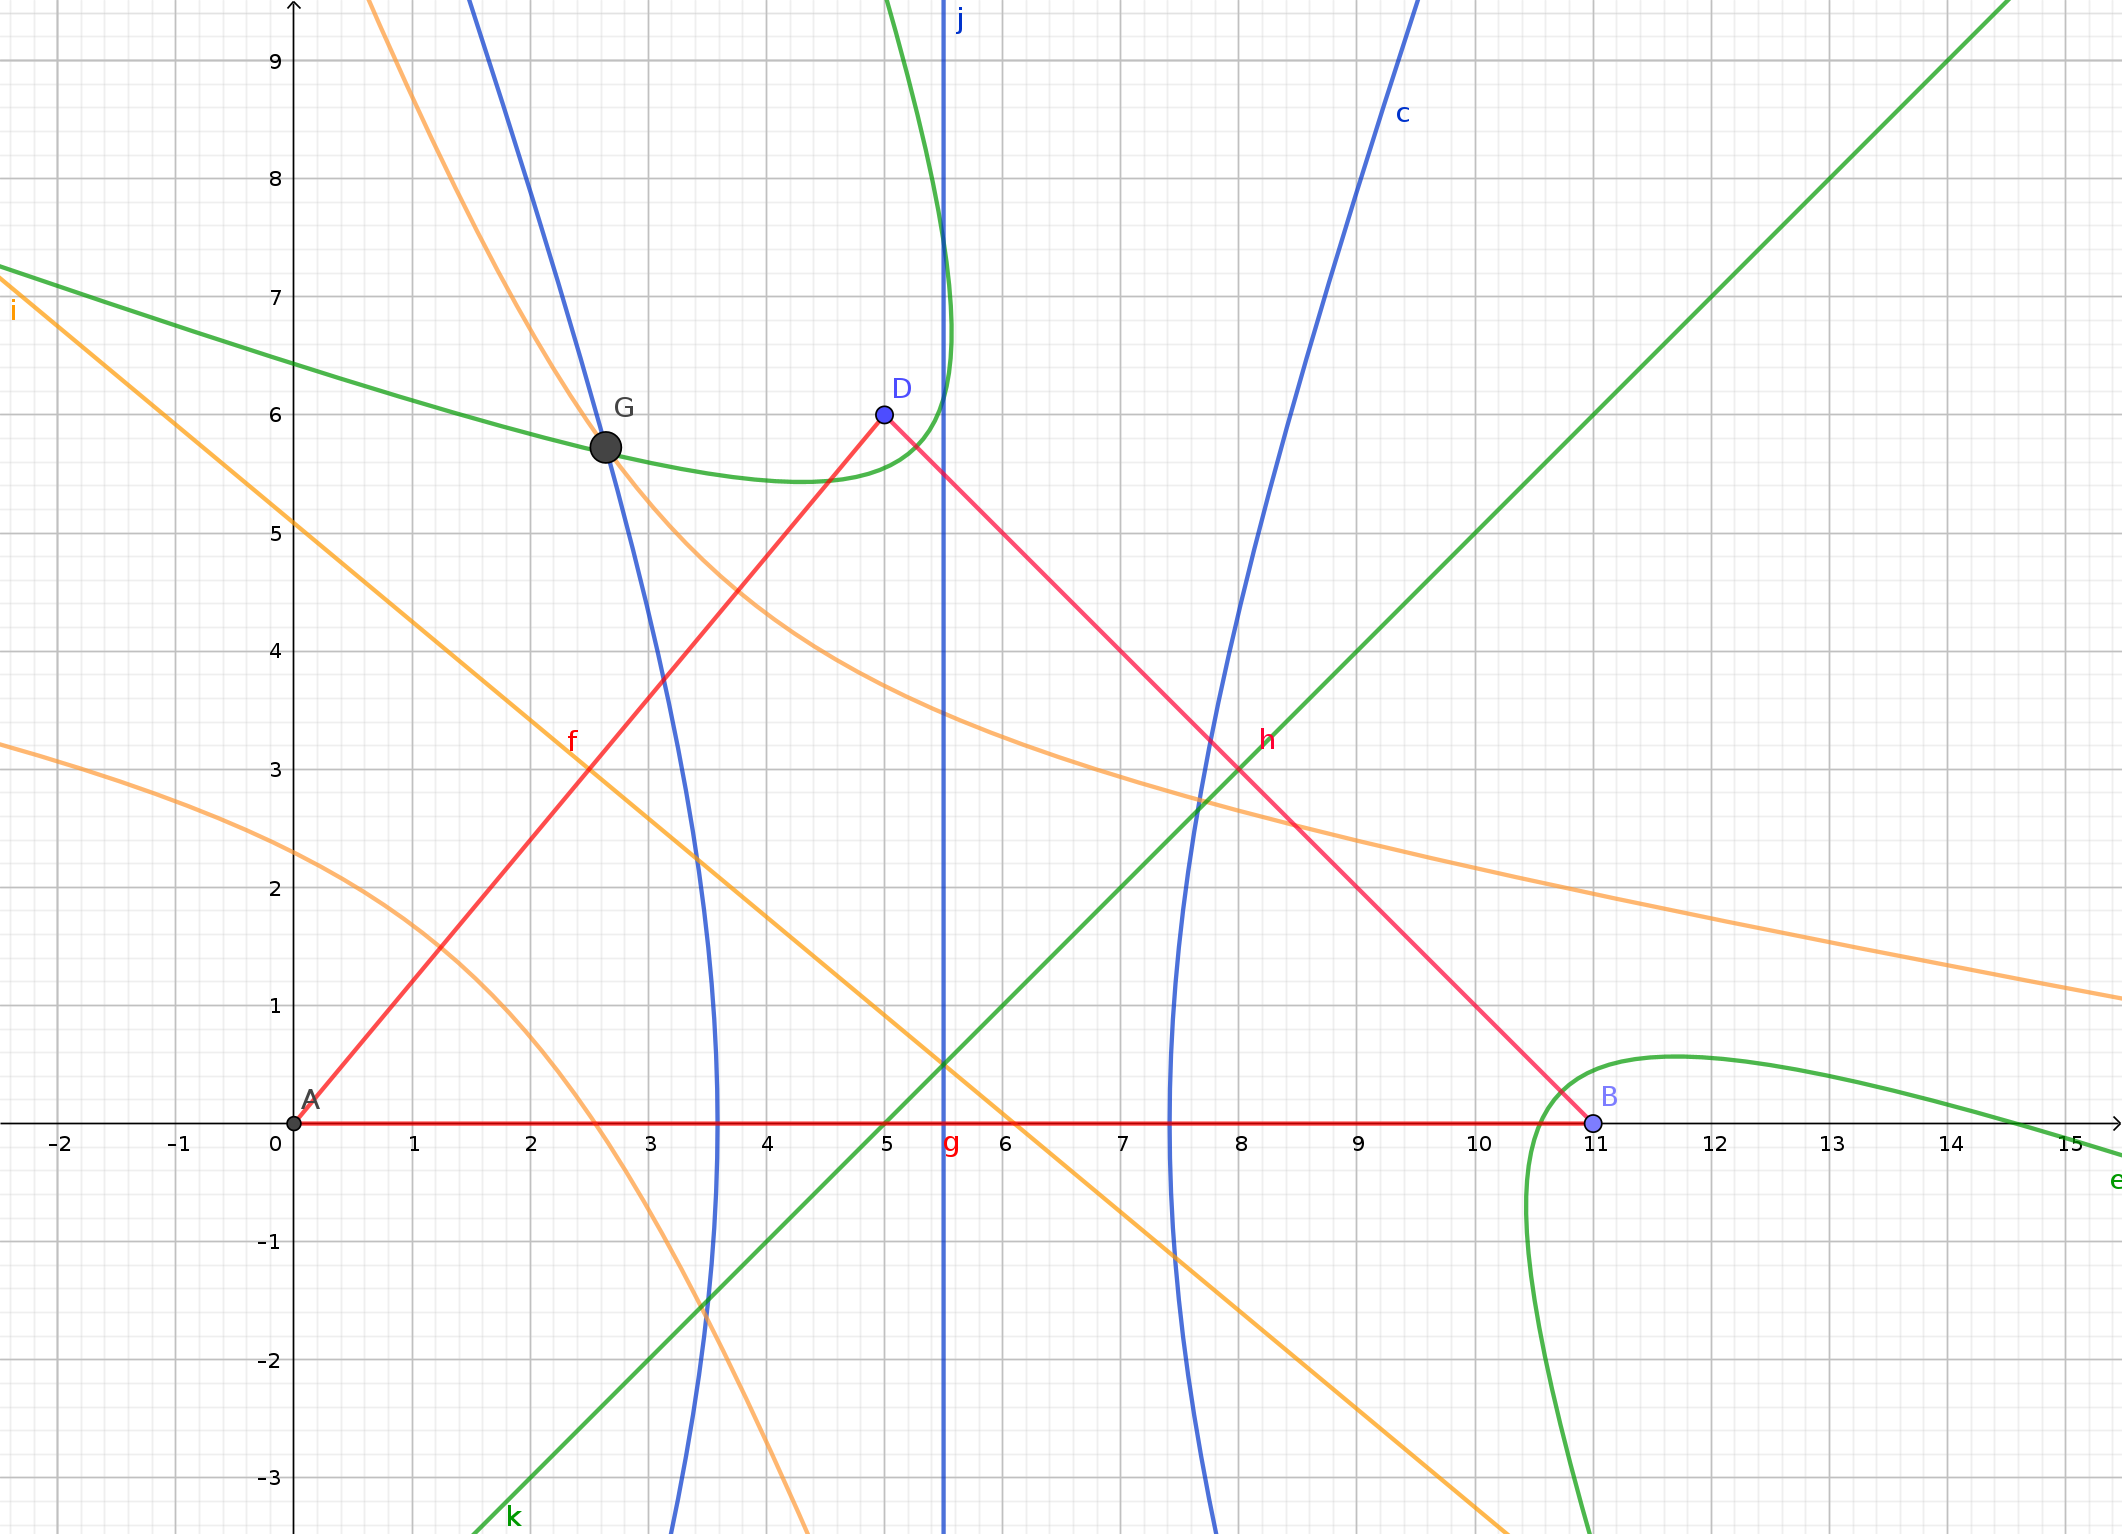
\includegraphics[width=0.9\textwidth]{tdoa.png}
    \caption{Time Difference of Arrival}
    \label{fig:tdoa}
\end{figure}

\subsection{Phase Difference of Arrival (PDoA)}
The PDoA method consists of combining the TWR scheme that delivers the distance between two devices with the measure of the bearing between the two devices. The combination of distance and bearing allows the calculation of the relative position of two devices without any other infrastructure. To do so, one of the devices carries two antennas and is able to measure the Phase Difference of Arrival of the RF signal.


Assume two antenna separated by a distance $d$, with a wavefront incident at an angle $\theta$, then the extra path the signal must travel between antenna 1 and antenna 2 (see figure \ref{fig:PhaseInterferometry}) results in a phase difference, \Delta\Phi, between the two antennas. This can be used to calculate the direction of arrival using:

\begin{equation}
    \theta = \arcsin(\frac{\lambda\Delta\Phi}{2\pi d})
\end{equation}

\begin{figure}[H]
    \centering
    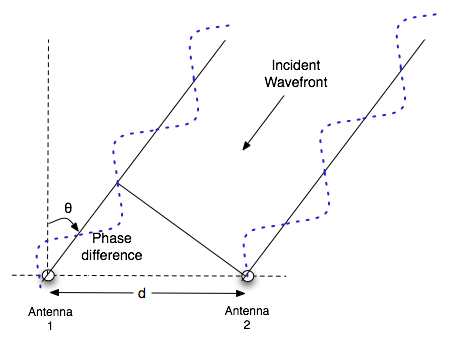
\includegraphics[width=0.7\textwidth]{PhaseInterferometry.png}
    \caption{Phase Difference of Arrival}
    \label{fig:PhaseInterferometry}
\end{figure}

\begin{figure}[H]
    \centering
    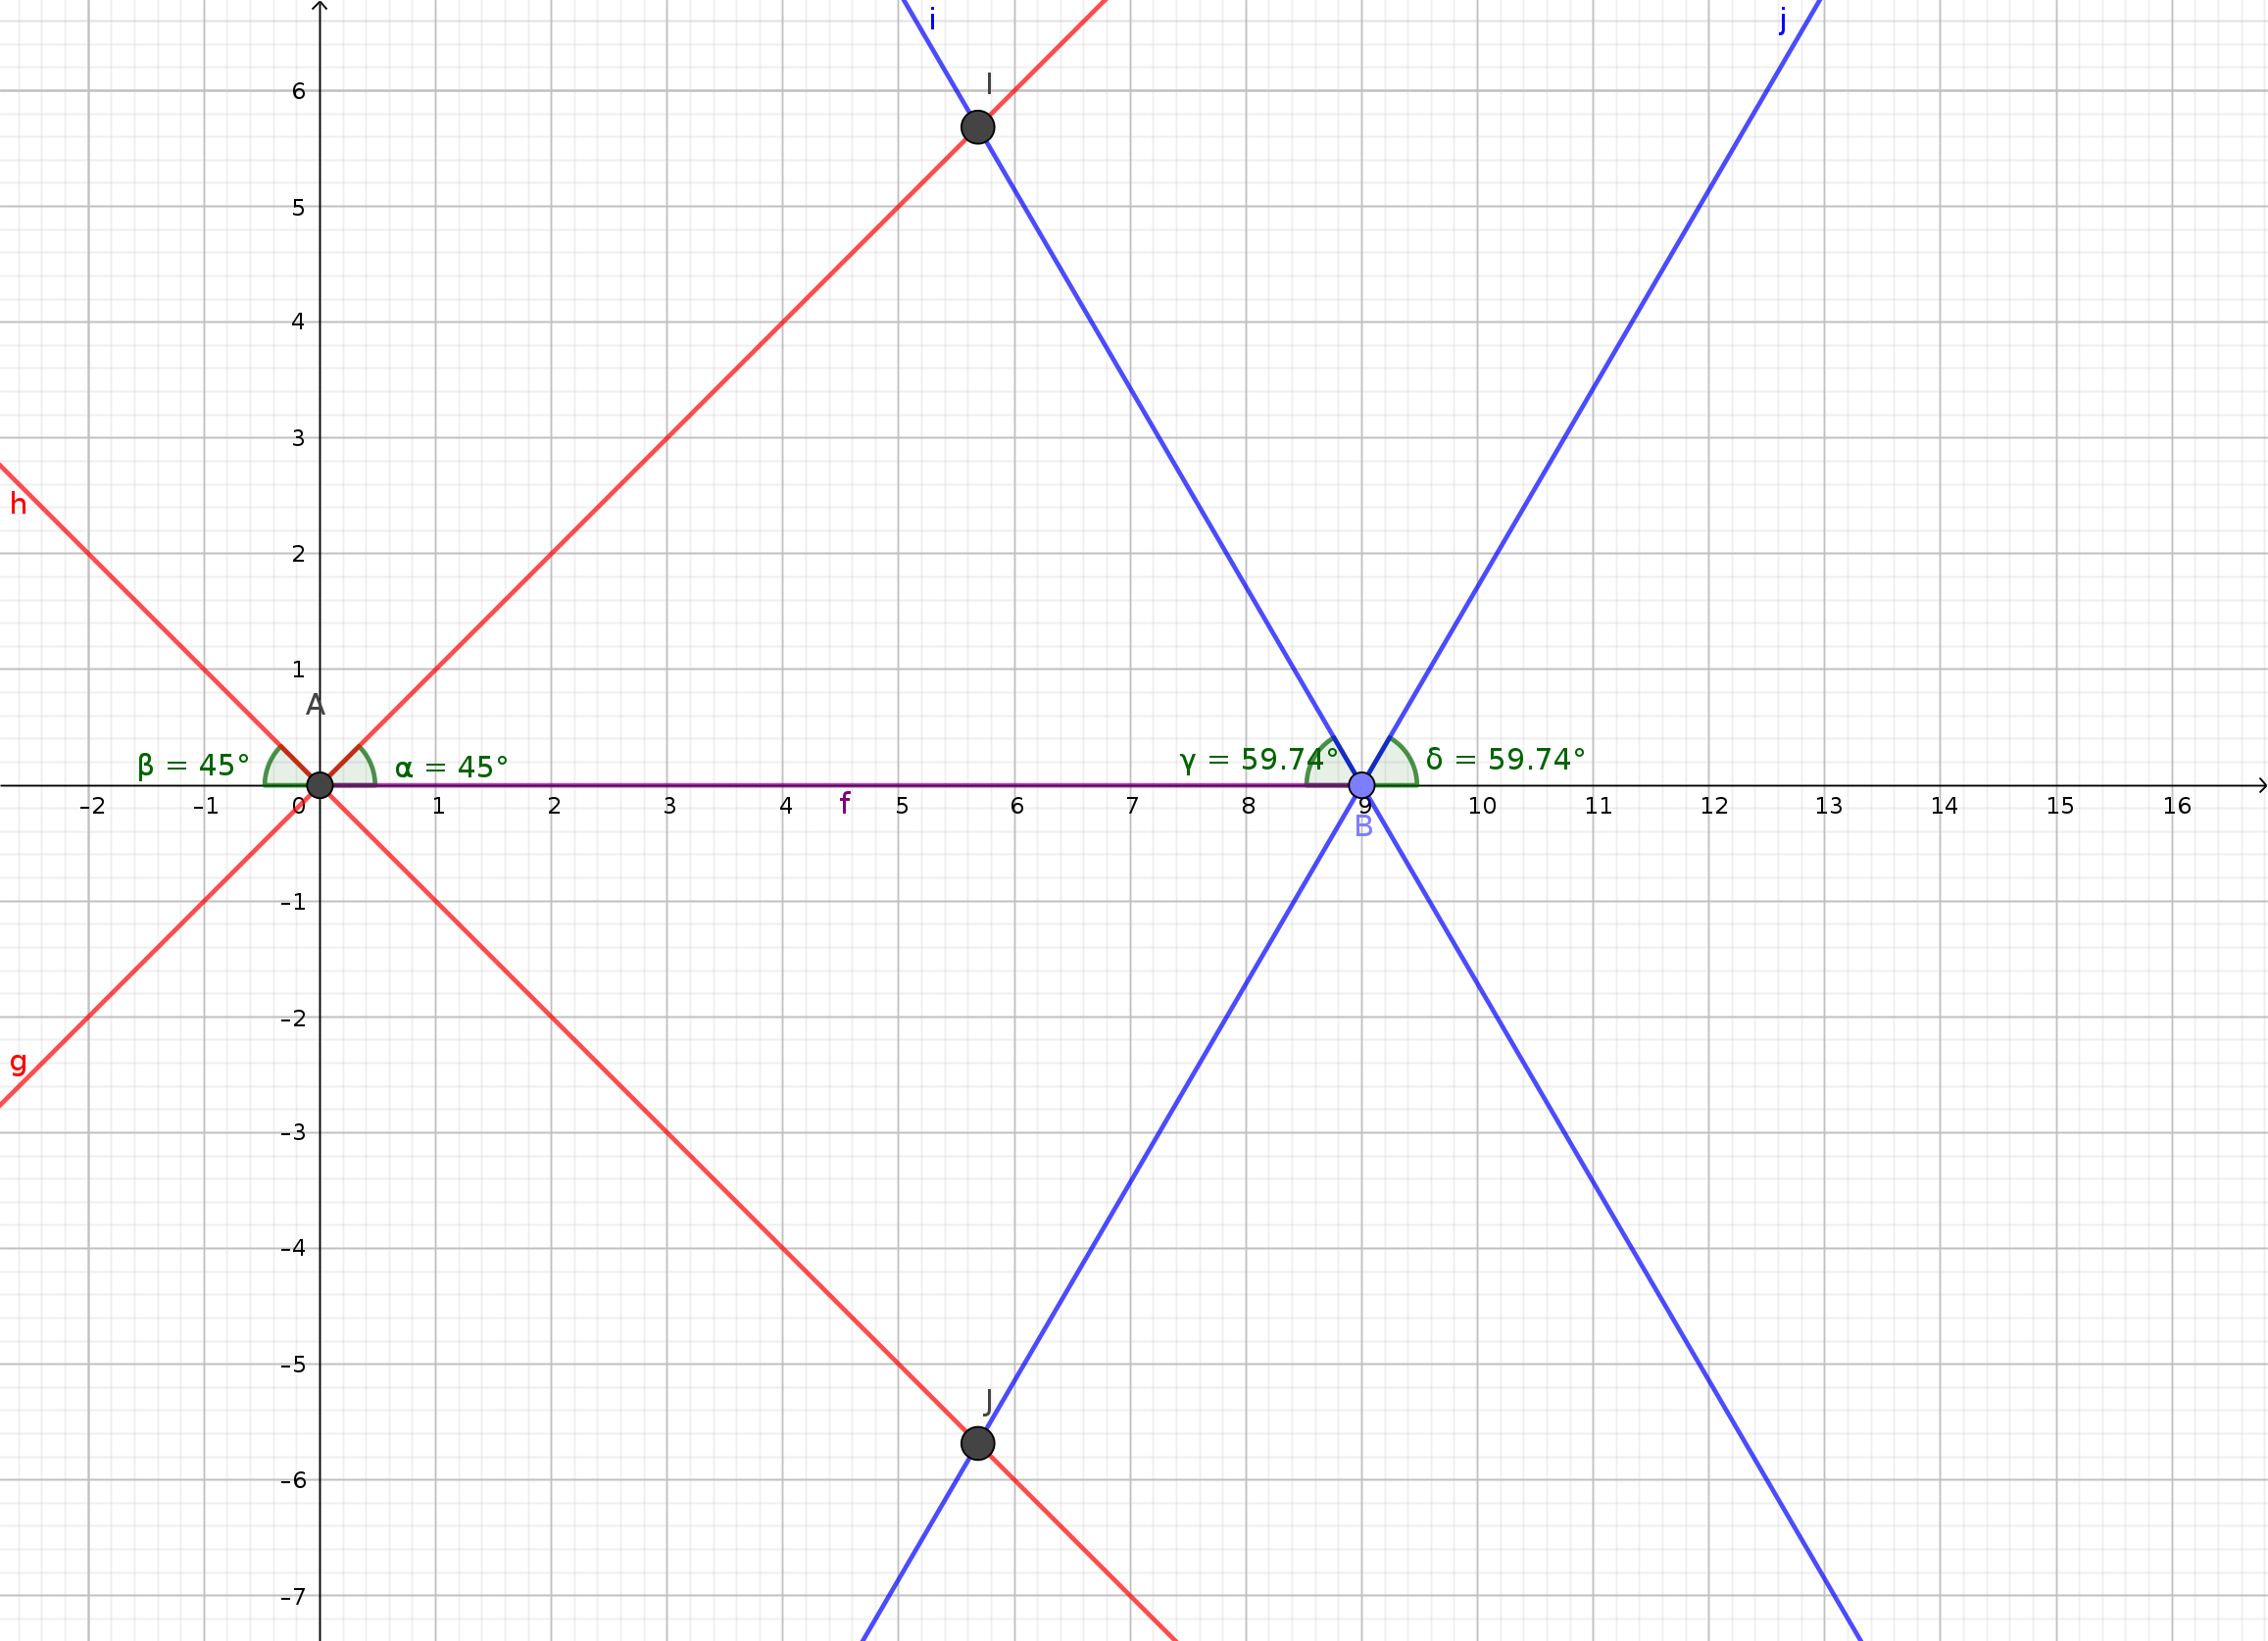
\includegraphics[width=0.9\textwidth]{pdoa.png}
    \caption{Phase Difference of Arrival}
    \label{fig:pdoa}
\end{figure}

\subsection{Two-Way Ranging (TWR)}
The TWR method relies on two-way communication between two devices. As they communicate, the devices also measure the Time of Flight of the UWB RF signal between them. By multiplying the round trip time of the signal by the speed of light, and then dividing by 2, you can derive the actual distance between the two devices. If you apply the TWR scheme between two devices, you will get the distance (D) between the two devices. Based on the TWR scheme, you can also implement 2D or even 3D location by measuring the distance between your mobile tags and fixed beacons – this is called triangulation.

\begin{figure}[H]
    \centering
    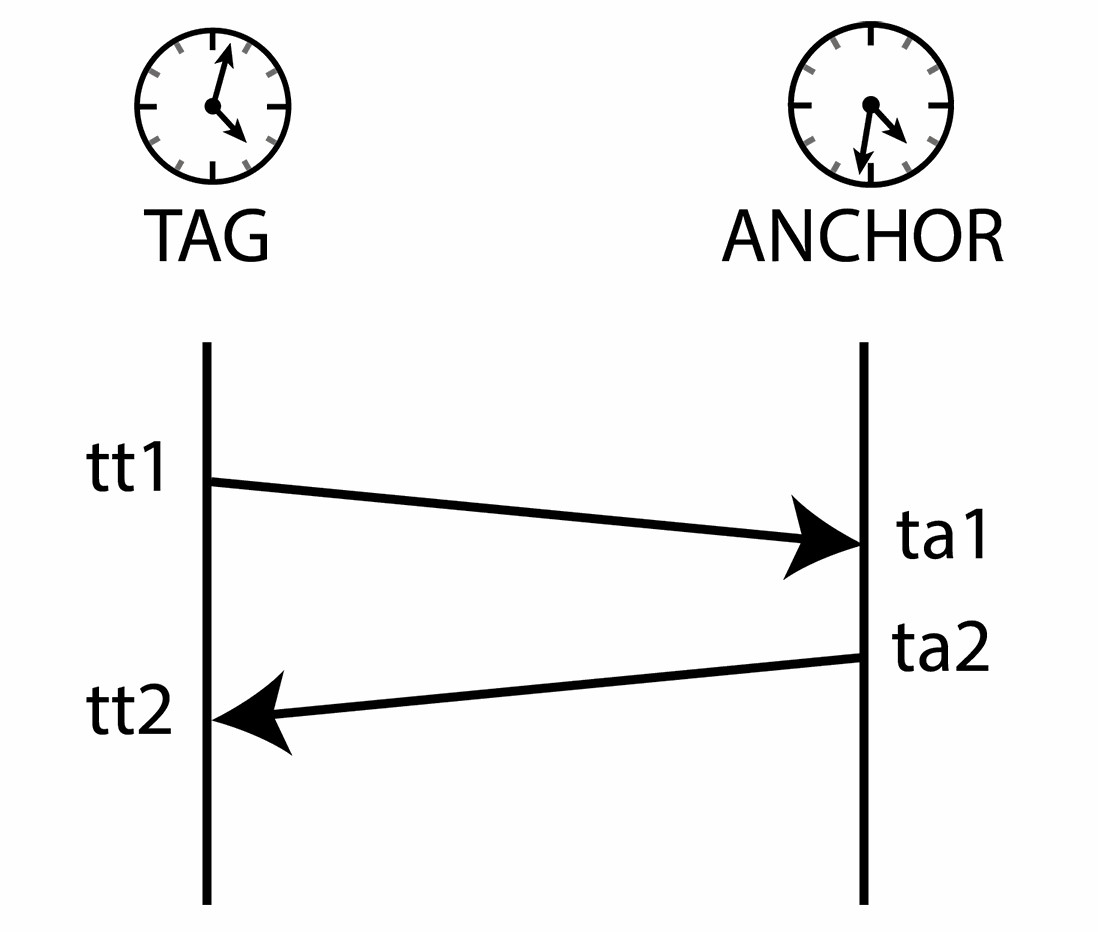
\includegraphics[width=0.3\textwidth]{twr_protocol.png}
    \caption{TWRImage}
    \label{fig:TWRImage}
\end{figure}

\begin{figure}[H]
    \centering
    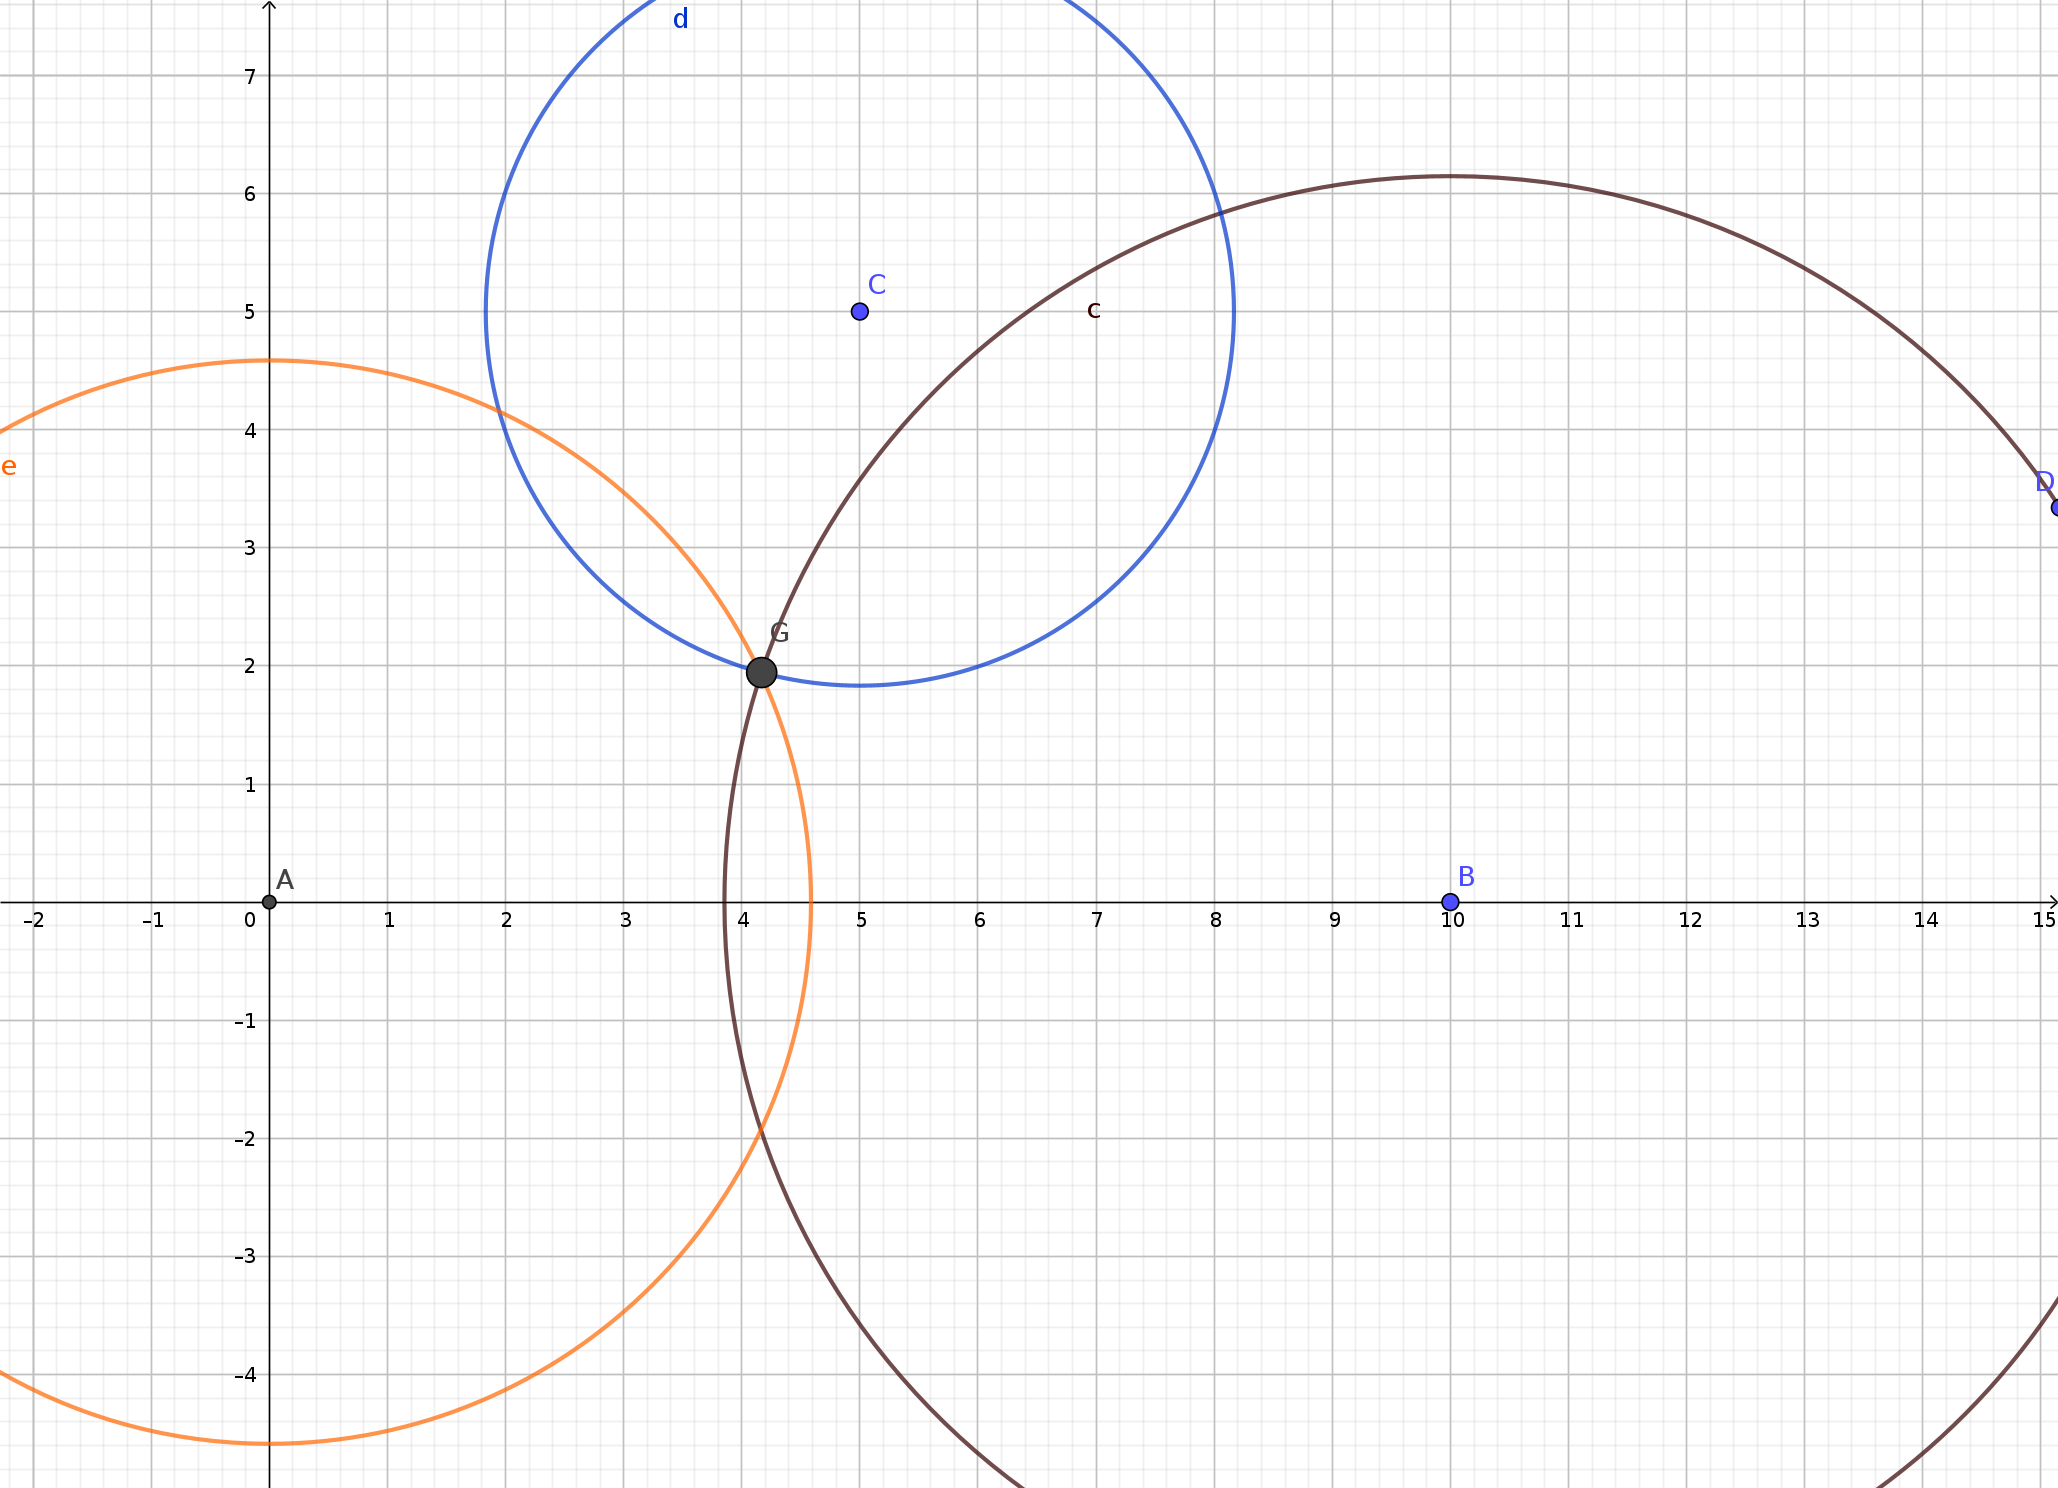
\includegraphics[width=0.9\textwidth]{twr.png}
    \caption{TWRImage}
    \label{fig:TWRImage}
\end{figure}

\section{Localization using trilateration}
\label{sec:localization_using_trilateration}

\end{document}